\section{2020 年 12 月 11 日答疑记录}


\begin{example}
    判断下列函数的奇偶性, 并求函数的零点.
    
    (1) $f(x)= x^{\frac12}$;\qquad
    (2) $g(x)= x+\dfrac1x$;\qquad
    (3) $h(x)= \mathrm{e}^x+\mathrm{e}^{-x}$;\qquad
    (4) $i(x)= \ln|x|$.
\end{example}
\begin{solution}
    (1) $f(x)= x^{\frac12}$ 的定义域为 $[0,+\infty)$, 不关于原点对称, 所以是非奇非偶函数. 令 $f(x)=x^{\frac12}=0$, 解得 $x=0$, 所以 $f(x)$ 的零点为 $0$.
    
    (2) $g(x)= x+\dfrac1x$ 的定义域为 $(-\infty,0)\cup(0,+\infty)$, 关于原点对称. 而 
    \[g(-x)= (-x)+\dfrac1{-x}= -\biggl(x+\dfrac1x\biggr)= -g(x),\]
    所以 $g(x)$ 是奇函数. 令 $g(x)= x+\dfrac1x= 0$, 得 $x^2+1=0$ ($x\neq 0$), 无解, 所以 $g(x)$ 没有零点.
    
    (3) $h(x)= \mathrm{e}^x+\mathrm{e}^{-x}$ 的定义域为 $\realnum$, 而
    \[h(-x)= \mathrm{e}^{-x}+\mathrm{e}^x= h(x),\]
    所以 $h(x)$ 是偶函数. 令 $h(x)= \mathrm{e}^x+\mathrm{e}^{-x}= 0$, 得 $(\mathrm{e}^x)^2+1=0$, 无解, 所以 $h(x)$ 没有零点. (注意, $h(x)$ 不是对勾函数, 其图形不像对勾.)
    
    (4) $i(x)= \ln|x|$ 的定义域为 $(-\infty,0)\cup(0,+\infty)$, 关于原点对称. 而 
    \[i(-x)= \ln|-x|= \ln|x|= i(x),\]
    所以 $i(x)$ 是偶函数. 令 $i(x)= \ln|x|= 0$, 得 $|x|=1$ 即 $x=\pm1$, 所以 $i(x)$ 的零点为 $\pm1$.
\end{solution}
\begin{remark}
    (1) 函数奇偶性的定义为
    \[\begin{aligned}
        \text{函数 $f(x)$ 的图形关于原点对称}
        &\Leftrightarrow\text{$f(x)$ 为奇函数}
        \Leftrightarrow f(-x)=-f(x),\\
        \text{函数 $f(x)$ 的图形关于 $y$~轴对称}
        &\Leftrightarrow\text{$f(x)$ 为偶函数}
        \Leftrightarrow f(-x)=f(x).
    \end{aligned}\]
    
    (2) 因为函数的奇偶性描述的是函数图形关于原点 (奇函数) 或 $y$~轴 (偶函数) 的对称性, 所以函数若有奇偶性, 则定义域必关于原点对称 (否则无法画出带对称性的图形).
\end{remark}

\begin{example}
    已知函数 $f(x)= \begin{cases}
        \dfrac1x, & x\geqslant 1,\\
        x^3, & x<1,
    \end{cases}$ 若关于 $x$ 的方程 $f(x)=k$ 有两个不等的实根, 求 $k$ 的取值范围.
\end{example}
\begin{solution}
    此题与 ``2020 年 12 月 5 日答疑记录'' 的例~\ref{exa:201217-1900} 类似, 画图可知, $k\in(0,1)$.
    
    \begin{center}
        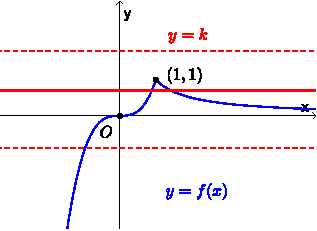
\includegraphics[scale=1]{2020-1217-1900-crop}
    \end{center}
\end{solution}


